%!TEX root = ../report.tex

% 
% Related work
% 

\section{Related Work}
\label{RelatedWork}

This section discusses standard organizations and benchmarking standards for FM. Also, an overview of existing benchmarking solutions such as ARCHIBUS and PNM Soft Sequence Kinetics is described. The scientific literature is also presented in this section along with a discussion of the normalization and prioritization of KPIs. 


\subsection{ISO and ICS}
The International Organization for Standardization (ISO) is the largest developer of voluntary International Standards covering all aspects of technology and business. ISO has formed joint committees to develop different kinds of standard according to the commission they join: IEC-International Electrotechnical Commission or ASTM-American Society for Testing and Materials. 
The International Classification for Standards (ICS) is a structure for catalogs of international, regional and national technical standards and other normative documents developed and maintained by ISO. It covers every economic sector and activity where these technical standards can be used. Its objective is to facilitate the harmonization of information and ordering tools \cite{ICS2005}.

Thus, we selected the most important standards for FM and Maintenance for those working with facilities in various stages of their life cycle, which are shown in Table \ref{tb:TableISO}, ordered by ICS.
\begin{landscape}
\begin{table}[h!]

		\centering
		\vspace{-2cm}
		\begin{adjustwidth}{0,5cm}{0cm}% adjust the L and R margins by 1 inch
		\resizebox{18cm}{!} {
			\begin{tabular}{ll}
				\hline
				{\bf Code} & {\bf Title} \\ 
				\hline

				{\bf ICS 01. 110: Facilities Management} &  \\
				ISO/CD 18480-1  & Part 1: Terms and definitions \\
				ISO/CD 18480-2  & Part 2: Guidance on strategic sourcing and the development of agreements \\
				\hline

				{\bf ICS 01. 110: Document Management} &  \\
				EC 82045-1:2001  & Part 1: Principles and methods \\
				IEC 82045-2:2004  & Part 2: Metadata elements and information reference model \\
				ISO 82045-5:2005 & Part 5: Application of metadata for the construction and facility management sector \\ 
				\hline

				{\bf ICS 03. 100: Risk Management} & \\
				ISO 31000:2009 & Principles and guidelines \\           
				ISO/TR 31004:2013  & Guidance for the implementation of ISO 31000 \\  		  
				IEC 31010:2009  & Risk assessment techniques \\  
				\hline

				{\bf ICS 03. 100: Asset Management}  & \\
				ISO 55000:2014 & Overview, principles and terminology \\ 	            
				ISO 55001:2014 & Management systems-Requirements \\		            
				ISO 55002:2014  & Management systems-Guidelines for the application of ISO 55001 \\  
				\hline

				{\bf ICS 03. 080: Outsourcing} & \\
				ISO/DIS 37500 & Guidance on outsourcing \\ 
				\hline

				{\bf ICS 91. 010: Building Information Modeling} & \\
				ISO/TS 12911:2012 & Framework for building information modeling (BIM) guidance \\ 		        
				ISO 29481-1:2010 & Information delivery manual-Part 1: Methodology and format \\	            
				ISO/AWI 29481-1 & Information delivery manual-Part 1: Methodology and format \\	            
				ISO 29481-2:2012 & Information delivery manual-Part 2: Interaction framework \\
				\hline

				{\bf ICS 91. 040: Buildings and Building Related Facilities}  & \\  
				ISO 11863:2011 & Functional and user requirements and performance -- Tools for assessment and comparison \\
				\hline

				{\bf ICS 91. 040: Buildings and Constructed Assets}  & \\
				ISO 15686-1:2011 & Service life planning-Part 1: General principles and framework \\
				ISO 15686-2:2012 & Service life planning-Part 2: Service life prediction procedures \\		            
				ISO 15686-3:2002 & Service life planning-Part 3: Performance audits and reviews  \\		            
				%ISO/CD 15686-5 & Service life planning-Part 5: Life-cycle costing  \\         
				ISO 15686-5:2008 & Service life planning-Part 5: Life-cycle costing  \\	            
				%ISO/AWI 15686--7 & Service life planning-Part 7: Performance evaluation for feedback of service life data from practice  \\		            
				ISO 15686-7:2006 & Service life planning-Part 7: Performance evaluation for feedback of service life data from practice  \\	            
				ISO 15686-8:2008 & Service life planning-Part 8: Reference service life and service--life estimation \\		            
				ISO/TS 15686-9:2008 & Service life planning-Part 9: Guidance on assessment of service--life data  \\		            
				ISO 15686-10:2010 & Service life planning-Part 10: When to assess functional performance \\		            
				ISO/DTR 15686-11 & Service life planning-Part 11: Terminology \\
				\hline

				{\bf ICS 91. 040: Buildings Construction}  &  \\
				ISO 15686-4:2014 & Service Life Planning -- Part 4: Service Life Planning using Building Information Modeling \\		            
				ISO 6242-1:1992 & Expression of users' requirements-Part 1: Thermal requirements  \\		            
				ISO 6242-2:1992 & Expression of users' requirements-Part 2: Air purity requirements  \\		            
				ISO 6242-3:1992 & Expression of users' requirements-Part 3: Acoustical requirements \\
				\hline

				{\bf ICS 91. 040: Performance Standards in Building}  & \\
				ISO 6240:1980 & Contents and presentation  \\	            
				ISO 6241:1984 & Principles for their preparation and factors to be considered  \\		            
				ISO 7162:1992 & Contents and format of standards for evaluation of performance  \\		            
				ISO 9699:1994 & Checklist for briefing-Contents of brief for building design  \\			            
				ISO 9836:2011 & Definition and calculation of area and space indicators \\
				\hline

			\end{tabular}
			}
		\end{adjustwidth}
		\caption{Specific ISO standards related to Facilities Management and Maintenance organized by ICS. The list presents the standards relevant for facilities in different stages of their life cycle.}
		\label{tb:TableISO}
\end{table}
\end{landscape}
In some ICS there are only ISO standards, in others, there are also European standards and national standards such as Portuguese national standards (NP). The latter are usually the transcripts for the Portuguese European legislative body (EN-NP)  or international (ISO-NP), but can also be standards developed from scratch in Portugal standards (in this case only have the designation NP). These can be consulted on Table \ref{tb:TableNPEN}.

\begin{table}[h!]
		\centering
		\vspace{0cm}
		\begin{adjustwidth}{0cm}{0cm}% adjust the L and R margins by 1 inch
			\begin{tabularx}{\textwidth}{l X}
				\hline
				\multicolumn{1}{l}{\bf Code} & \multicolumn{1}{l}{ \bf Title} \\ 
				\hline

				{\bf Facilities Management} & \\
				EN 15221-1:2006 & Part 1: Terms and definitions \\
				EN 15221-2:2006  & Part 2: Guidance on how to prepare facility management agreements \\
				EN 15221-3:2011  & Part 3: Guidance on quality in facility management \\
				EN 15221-4:2011  & Part 4: Taxonomy, classification and structures in facility management \\
				EN 15221-5:2011  &  Part 5: Guidance on facility management processes \\
				EN 15221-6:2011  &  Part 6: Area and space measurement in facility management \\
				EN 15221-7:2012  &  Part 7: Guidelines for performance benchmarking\\
				\hline

				{\bf Maintenance Management} &  \\
				NP EN 13269:2007  & Instructions for maintenance contract preparation \\
				 NP EN 13460:2009 & Maintenance documentation \\
				NP EN 15341:2009  &  Maintenance key performance indicators (KPI) \\ 
				NP 4483:2009  & Guide for maintenance management system implementation \\ 
				 NP 4492:2010 & Requirements for maintenance services \\ 
				 EN 13306:2010  & Maintenance terminology \\ 
				 EN 15331:2011 & Criteria for design, management and control of maintenance services for buildings \\ 
				CEN/TR 15628:2007 & Qualification of maintenance personnel \\ 
				EN 13269:2006  & Guideline on preparation of maintenance contracts \\ 
				\hline

			\end{tabularx}
		\caption{List of European (EN) and Portuguese (NP) FM and Maintenance Standards that apply to facilities in various stages of their life cycle. }
		\label{tb:TableNPEN}
		\end{adjustwidth}
\end{table}

\subsection{Benchmarking Standards for FM}

The importance of standards resides in the creation of specifications, which normalizes how some activity is performed. In the case of benchmarking, standardizing how companies evaluate their FM data enables compatibility between organizations, and so, there is no misinterpretation between different organizations for a given measurement. 

Becomes possible to compare the results between them, which empowers an improvement and enhancement of facilities management for each organization. Accordingly, it is essential to have specific standards of measurement and metrics for ensuring a common understanding of performance and to identify performance gaps \cite{Mass1998}.

Various FM software from many organizations tend to use ISO standards and Royal Institution of Chartered Surveyors (RICS) measurement practices. 

\subsubsection{RICS and BICS Space Measurement Normalization}

\hfill \\ \\ There are many standards that specify how to perform measurements, so that it can be executed equally by the different organizations. Thus, measurements must be performed by accredited specialists in the matter, such as Chartered Surveyors that are professionals members of the Royal Institution of Chartered Surveyors (RICS) and that can offer impartial, specialist advice on a variety of property related issues.

RICS has a Code of Measurement Practice that deals with practice of measurements such as valuation techniques (zoning of shops) or special uses. It specifies measurements for 
\begin{enumerate*}[label=\itshape\roman{enumi})]
	\item Gross External Areas (GEA): area of a building measured externally at each floor level, 
	\item Gross Internal Areas (GIA): area of a building measured to the internal face of the perimeter walls at each floor level 
	\item p: area within a perimeter walls at each floor level
\end{enumerate*} \cite{RICS2007}.
RICS provides precise definitions to permit the accurate measurement of buildings and land or the calculation of sizes (areas and volumes) presented in the RICS' Code of Measuring Practice \cite{RICS2007}. %, and is just one example of an institution which regulate standards. 

Belonging to RICS, the   (BCIS) provides built environment cost information, and is the basis of early cost advice in construction industry, since they provide services respecting occupancy costs, construction duration, repair costs, construction inflation, among others. 
Today, the focus is to deliver buildings to a known cost and on being able to track the reduction in costs that result from improvements in procurement \cite{BCIS2008}. For this to happen, it is necessary information provided by BCIS such as cost per $m2$ of Gross Internal Floor Area for buildings and elements.

BCIS elemental cost data usefulness is reinforced by the changing procurement methods, the changing means of information management and the growing need for through life data. Also, with the development of BIM, it is necessary that information from the BIM model be supplied at various stages along the project time line, in order that the costs can be produced and validated. This information, derived from a block model, will provide basic quantities from which element unit quantities can be derived.

The BCIS Elemental Standard Form of Cost Analysis \cite{BCIS2008} describes the rules for preparing an elemental cost analysis in standard BCIS format, and it describes the principles of analysis, instructions on the information required to complete a costs analysis, general definitions, definitions of the elements and sub-elements, and element unit quantities \cite{BCIS2008}.

%There are some important principles of analysis such as
%\begin{enumerate*}[label=\itshape\roman{enumi})]
% 	\item each building within a project should be analysed separately 
% 	\item the costs analysed should be the agreed price for the works described,
% \end{enumerate*} and some levels such as
% \begin{enumerate*}[label=\itshape\roman{enumi})]
% 	\item Total Building (building, external works)
% 	\item Group Elements (substructure, superstructure, internal finishes, prefabricated buildings or buildings units)
% 	\item Detailed Elements 
% 	\item Sub-elements
%\end{enumerate*}.

As referred in the BCIS Elemental Standard Form of Cost Analysis, there has to be detailed information documents about the projects, buildings, procurements, costs (there should be provided Total Costs for each element and sub-elements, and should be shown separately when required and for different forms of construction), risks and design criteria.
\subsubsection{IFMA Benchmarking}
\hfill \\ \\ The International Facility Management Association (IFMA) has developed a facility benchmarking useful for current FM services benchmarking that can be seen in Figure \ref{fig:IFMAMethodology} as shown in the report \cite{Roka-Madarasz2010}.


\begin{figure}[t!]

  \centering
  \begin{adjustwidth}{-0,6cm}{0cm}
  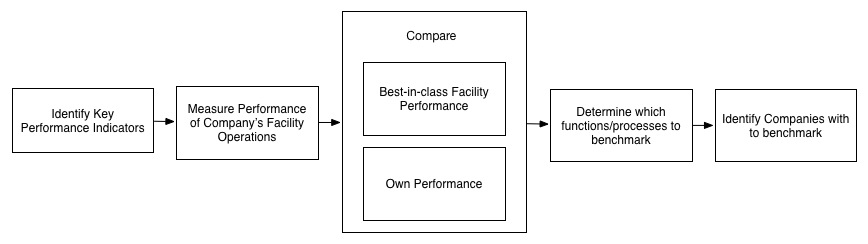
\includegraphics[width=1.1\textwidth]{img/IFMAMethBenchProcess.jpg}
  \end{adjustwidth}
  \caption{IFMA Benchmarking Methodology adapted from Roka-Madarasz \cite{Roka-Madarasz2010}. First step is to identify the KPI, then, use it to measure the facility performance. At this point three different paths can be taken: Best-in-class Facility Performance, Own Performance, or directly to Compare. After this, the functions of benchmark has to be chosen, just like which companies to benchmark.}
  \label{fig:IFMAMethodology}
\end{figure}

In order to measure facilities performance, IFMA has established 9 Key Performance Indicators that must be easily measurable and that must be defined for monitoring the actual process and also to control it. These Key Performance Indicators shown in the report \cite{Roka-Madarasz2010} can be seen in Table \ref{tb:TableKPIFMBenchmarking} on Appendix.

% \subsubsection{BOMA}

% \hfill \\ \\ The Building Owners and Managers Association (BOMA International) is a organization for commercial real estate professionals such as building owners, managers, developers, leasing professional, products and services providers, etc. It is a federation of 93 BOMA U.S. associations, BOMA Canada and its 11 regional associations and 13 BOMA international affiliates.

% Its objective is to advance the interests of the entire commercial real estate industry through advocacy, education, research, standards and information, so, BOMA monitor and lobby pertinent legislative, regulatory and codes/standards issues (electricity deregulation, capital gains tax relief, telecommunications, indoor air quality, etc). 

% BOMA International is a primary source of information on building management and operations, development, leasing, building operating costs, energy consumption patterns, local and national building codes, legislation, occupancy statistics, technological developments and other industry trends.

\subsection{Existing Solutions}

As specified in section \ref{FacilitiesManagement}, there are many types of softwares for FM solutions, like CAFM or IWMS. All of known FM solutions like Maxpanda \cite{maxpanda} or IBM Tririga \cite{IBMtririga} are a simpler way to manage facilities, they centralize organizations information, making management more efficient through business analytics, critical alert, increasing visibility and control.

Some of them, like ARCHIBUS \cite{ARCHIBUSsite} or FM:Systems \cite{FMsystems} have integration with CAD or BIM models, which is very important for visualization of departments occupation or others space and occupation management areas. 

Most of these systems promotes their capabilities for organizations cost reduction --- since they cost-justify real changes in preventive maintenance routines and predicts cost effects of preventive maintenance changes before they are made --- some permits multiple users, others make possible that each user only can access specific information regarding his organization position.

There are different sectors that a FM system can focus like 
\begin{enumerate*}[label=\itshape\roman{enumi})]
	\item Capital/ Financial,
	\item Real Estate/Retail: Construction or Project Management,
	\item Space and Workplace, 
	\item Maintenance, 
	\item Sustainability and Energy,
	%\item Document, 
	\item Move,
	%\item Facilities,
	\item Higher Education and Public 
\end{enumerate*}. Many of the existent solutions only focus in some of this sectors and not in all of them.

For Real Estate it is usual features for incorporation of current lease accounting standards, tracking of dates and contractual commitments, management of occupancy and facilities costs. 
On Capital/Finantial are being used features to identify funding priorities within capital programs, reduce project schedule overruns or streamline project cost accounting.
In Space and Workplace it is important to have tools for space use agreements and chargeback to increase departmental accountability for space use.
Maintenance requires features for automatically route and manage both incoming and planned maintenance, while at the same time keeping internal customers up to date on the progress of their work tickets, or streamline facility maintenance, service management and facility condition assessments. 
The Sustainability and Energy sector is also very important for defining which projects will achieve the right mix of environmental benefits and cost savings, for reduce energy consumption to meet sustainability goals, identifying poorly performing facilities and automate corrective actions.

Systems like Indus System \cite{IndusSystems}, Manhattan Mobile Apps \cite{ManhattanAppMobile}, PNMSoft \cite{pnmSoftsite} or ARCHIBUS have cloud-based software that enables users to access FM systems anywhere on mobile devices from a browser.
Indus System enables users to store, share, view drawings, space, assets, related costs, leases and contracts just by accessing the browser.

For other hand, ARCHIBUS and PNMSoft are both capable of showing an organizations KPIs through their web site. The packages enables users normal usage of their daily management software and then, when necessary, the visualization of the results on a graphical web application.
However, this solution is only applicable for the facilities that have ARCHIBUS or PNMSoft software installed, and only for comparison from previous results from that facility.
In contrast, with our solution, any organization could benefit from this features and one more: the comparison with others organizations on the sector.

\subsubsection{ARCHIBUS}

\hfill \\ \\ ARCHIBUS is the provider Facilities Management software solution that effectively tracks and analyzes not only facilities-related information but also real-estate. ARCHIBUS is an integrated solution that applies to organizations of all sizes and sectors (here we focus on ARCHIBUS for Educational Institutions reports - Table \ref{tb:ARCHIBUSListActReports} on Appendix).

The system architecture consists of three main modules (as seen on Figure \ref{fig:ArchiModules}), the first, is named ARCHIBUS Web Central and provides live enterprise access to facilities data and enables the easy maintenance and distribution of facilities information across the entire enterprise \cite{ARCHI}. A role-based security service, allows that when users log on, they only access information relevant to their roles on the organization.

\begin{figure}[t!]
  \centering
  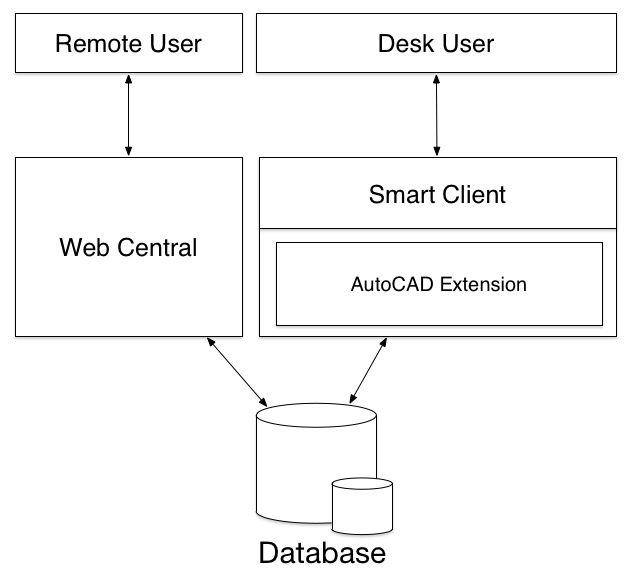
\includegraphics[width=0.50\textwidth]{img/ARCHIBUSModules.jpg}
  \caption{Overview of ARCHIBUS software architecture adapted from ARCHIBUS Fundamentals Training \cite{ARCHI}. The Database is the same for all modules, so the data is coherent between them. Module Extension for AutoCAD is only applicable for the module Smart Client, that can only be used by Desk Users. Remote users that are not on the office, can use Web Central to access data.}
  \label{fig:ArchiModules}
\end{figure}
 
ARCHIBUS have a .NET Windows application, named Smart Client, used by back-office personnel for data entry, data transfer, importing and exporting data from other systems. This module has another one integrated, the Smart Client Extension for AutoCAD or DWG Editor that is very important for those organizations who want to include Computer-Aided Drawing or BIM models.  

From a technical standpoint, the software architecture of ARCHIBUS consists of a database that can be one of MS SQL, Oracle or Sybase. This database communicates with the application servers that can run on Tomcat, Jetty, WebLogic or WebSphere. The applications of SmarClient module running on the computer of the client companies, communicate with application servers through Web Services and the applications of Web Central module communicates via HTTP with those same servers \cite{ARCHI}.

Being part of the ARCHIBUS platform, ARCHIBUS Performance Metrics Framework delivers KPIs and other performance data about the real estate, infrastructure and facilities using a detailed graphical view of the data. Thus, it is possible to use analytical measures and productivity tools, which provides decision-makers to align their portfolio to organizational strategy, spotlight underperforming business units or assets, and benchmark organizational progress to achieve targeted goals.

\subsubsection{PNM Soft Sequence Kinetics}

\hfill \\ \\ PNM Soft Sequence Kinetics is an Intelligent Business Process Management Suite and covers process optimizing KPI, dynamic process change, KPI analysis, process operation and tracking, communication with external systems and mobile and cloud KPI.

This system has four main focus: Processing-Optimizing KPI, Process Operation and Visual Tracking, KPI for Process Administrators and Mobile Process KPI.

On the Process Optimizing KPI there are two different processes: 
\begin{description}
	\item  [Extra-Process Performance Analytics] permits the process performance tracking via runtime dashboards and displays KPI like process status levels or average execution time of a process, which helps to understand how successful the process is and highlight required improvement areas.\\

	\item  [Intra-Process Analytics] aggregation and calculation of intra-process data by real-time analytics, that is built into the Business Rule editor, which enables routing according to their results via a simple GUI, being an artificial process intelligence form which sees the business teach itself how to perform better over time.
\end{description}

Process Operation and Visual Tracking is possible by Flowtime that is a extension of Microsoft SharePoint with a built-in process operation environment, which enables the collaboration on processes in a familiar interface and includes advanced task management, delegation and monitoring of KPI capabilities with a tracking views, which shows the process stands.

The KPI for Process Administrators provides important indicators on process performance per type of process \cite{PNMSOFT}.

PNM Soft also has a mobile application named Mobile Portal, that is available as an application or an online service, where users can access the same features provided by Sequence Kinetics Flowtime and can be configured by the customer to meet his necessities. 
For the cloud platform PNM Soft uses Windows Azure.

\subsection{Scientific Literature} \label{ScientificStudies}

Ho et al \cite{Ho2000} report different performance measurements and indicators most used in Asia Pacific region. This research work rates the importance of 97 metrics on a five point scale and indicate if the metric was being used in their organization FM --- the metrics consisted of performance measurements and performance indicators grouped by eight categories:
\begin{enumerate*}[label=\itshape\roman{enumi})]
 	\item size and use of facilities,
 	\item maintenance,
 	\item refurbishment,
 	\item cleaning,
 	\item energy consumption,
 	\item ground and environment,
 	\item safety and security,
 	\item parking.
\end{enumerate*}
These categories are represented by order of importance on Figure \ref{fig:MeasurementCatPriority}, according to the study by Ho et al \cite{Ho2000}.
% \begin{table}
% 	\begin{adjustwidth}{4,5cm}{0cm}
% 	\begin{tabular}{l}
% 		\multicolumn{1}{c}{\bf Category} \\
% 		\hline
% 		Cleaning \\
% 		Refurbishment \\
% 		Parking \\
% 		Ground and Environment \\
% 		Size and use of facilities \\
% 		Safety and Security \\
% 		Maintenance \\
% 		Energy Consumption \\	
% 		\hline
% 	\end{tabular}
% 	\end{adjustwidth}
% \caption{Measurement Categories ordered by their importance according to the results of the research of Ho et al \cite{Ho2000}.}
% \label{tb:CategoriesHo}
% \end{table}

\begin{figure}[t!]
  \centering
  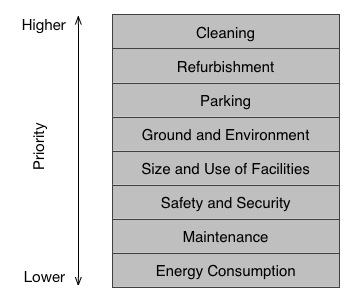
\includegraphics[width=0.40\textwidth]{img/MeasurementCatPriority.jpg}
  \caption{Measurement Categories ordered by their importance according to the results of the research of Ho et al \cite{Ho2000}.}
  \label{fig:MeasurementCatPriority}
\end{figure}



Moreover, Ho et al \cite{Ho2000} also identified which of the 97 metrics were the most used and more important to the organizations: the metrics that lead a direct financial implication were the ones with a higher rating. The 30 metrics with higher rates are especially related to the areas of:
\begin{enumerate*}[label=\itshape\roman{enumi})]
 	\item Financial such as Total Annual Facility Cost and Operational Cost, 
 	\item Spacial such as Gross Floor Area/Usable Floor Area and Usable Area,
 	\item Maintenance such as Asset Replacement Value (Maintained),
 	\item Cleaning such as Area Cleaned and Cleanliness Status of Site.
\end{enumerate*}

% \begin{enumerate*}[label=\roman{enumi})]
% 	\item Total Annual Facility Cost,\\
% 	\item Total Maintenance Expenditure,\\
% 	\item Total Cleaning Cost,\\
% 	\item Initial Cost,\\
% 	\item Operation Cost,\\
% 	\item Cleaning Expenditure/m2,\\
% 	\item Total Refurbishment Value (total),\\
% 	\item Annual Income,\\
% 	\item Gross Floor Area/Usable Floor Area,\\
% 	\item Cleanliness Status of Site, Interior and Exterior and Fittings, etc,\\
% 	\item Annual Consumption,\\
% 	\item Gross Floor Area,\\
% 	\item Competence of in-house staff,\\
% 	\item Adequacy of Budget,\\
% 	\item Annual Cost of Energy Purchased,\\
% 	\item Total Number of Parking Spaces Available,\\
% 	\item Usable Area,\\
% 	\item Rentable Area,\\
% 	\item Operation Cost/m2,\\
% 	\item Occupants Satisfaction,\\
% 	\item Frequency of Building Failures,\\
% 	\item Facility Budget/Corporation Budget,\\
% 	\item Asset Replacement Value (Maintained),\\
% 	\item Cost per m2,\\
% 	\item Total ground Maintenance Expenditure,\\
% 	\item Total Environment Cost,\\
% 	\item Occupancy Cost/m2,\\
% 	\item Facility Budget/Facility Assets,\\
% 	\item Area Cleaned.
% \end{enumerate*}

Massheder and Finch \cite{Mass1998}, surveyed the FM benchmarking metrics used in the UK. Their work identified which metrics were used to measure performance of the FM function. They organized metrics according to five categories:
\begin{enumerate*}[label=\itshape\roman{enumi})]
	\item business metrics,
	\item building performance metrics,
	\item portfolio metrics,
	\item acquisition  metrics,
	\item disposal metrics. 
\end{enumerate*} The results of their study are presented in Table \ref{tb:TableUseBenchmarkingMetrics}. As we can see, the most used metrics are the Business, Portfolio Metrics and Building Performance. The latter is considered the most important one (with percentage of use above 50\% on 5 of 6 metrics presented.)

\begin{table}[h!]
	\vspace{0cm}
	\begin{adjustwidth}{-0,5cm}{0cm}
	\begin{tabular}{l r}
		\hline
		\multicolumn{1}{l}{\bf Metric} & \multicolumn{1}{r}{ \bf Percentage of Use } \\ 
		\hline

		{\bf {\emph{Business}}} & \\
		Occupancy cost of operating revenue by building &  43\% \\
		Occupancy cost of the total of labour and costs by business unit &  29\% \\
		Occupancy of cost of operating revenue by business unit &  21\% \\ 
		Occupancy cost of the total sales and admin cost by business unit  &  14\% \\ 
		Location analysis on basis of where key skills are available & 7\% \\ 
		Location optimization (in context of attractors and repellers) &  7\% \\ 
		\hline

		{\bf {\emph{Building Performance}}} & \\
		Occupancy cost per $m^2$ &  98\% \\
		Occupancy cost per person &  79\% \\
		Occupancy of cost per building size &  64\% \\ 
		$m^2$ per person  &  64\% \\ 
		Itemized (occupancy) cost comparisons of $m^2$ per person by building & 36\% \\ 
		Absentee rates by building &  0\% \\ 
		\hline

		{\bf {\emph{Portfolio Metrics}}} & \\
		Proportion of operational space compared to non-operational space &  49\% \\
		Current market capital value compared to book value by building &  21\% \\
		Current market rental value compared to rent peasing by building &  14\% \\ 
		Proportion of Non-operational Space that is Sublet or Assigned  &  14\% \\ 
		\hline

		{\bf {\emph{Acquisition Metrics (only those who include real estate in FM)}}} & \\
		Costs of acquisition measured against returns &  20\% \\
		Actual extra occupancy cost against prediction cost &  10\% \\
		Amount of space coming on stream per unit time &  10\% \\ 
		Time to find and acquire space against program &  10\% \\ 
		Time to occupation against program & 10\% \\ 
		\hline

		{\bf {\emph{Disposal Metrics (only those who include real Estate in FM)}}} & \\
		Holding costs per year &  30\% \\
		 Time to dispose of buildings against program &  30\% \\
		 Cost of disposal against savings &  20\% \\ 
		Time to clear buildings against program  &  20\% \\ 
		 Holding costs to lease end, break and/or estimated disposal date & 10\% \\ 
		 Number of months vacant to date &  10\% \\ 
		 Disposal performance measures against natural portfolio shed rate & 0\% \\ 
		 Months vacancy to lease end, break and/or estimated disposal date &  0\% \\ 
		\hline

	\end{tabular}
	\end{adjustwidth}
\caption{Use of the different metrics on UK benchmarking organizations according to Massheder et al \cite{Mass1998}. The most used metrics are the ones belonging to Building Performance, Business and Portfolio with a percentage of use above the Acquisition and Disposal categories.}
\label{tb:TableUseBenchmarkingMetrics}
\end{table}

%Gilleard and Yat-lung (2004) suggested applying Analytic Hierarchy Process (AHP) to FM benchmarking. AHP, designed in 1970 by Saaty, helps decision-makers set priorities and make best decision when both qualitative and quantitative aspects of decision need to be considered, making complex problems into small ones \cite{Gilleard2004}.
%After their study, they arrived at a conclusion that applying AHP to FM benchmarking helps facility managers to assimilate all the facts, weight the pros and cons and communicate the performance benchmarks in a logical manner \cite{Gilleard2004}.


Hinks and McNay \cite{Hinks1999} identified a need to established a set of universally accepted KPI that realistically evaluate organizations performance.  
On their study, they identified the need to clarify and prioritize the parameters and indicators which correlated the views of the customer and the departments, to support the operational requirements of the core financial business. To this end, they used the Delphie technique \cite{Eynde1997} (used to gather expert opinion in areas where there is considerable uncertainty and/or lack of agreed knowledge \cite{Hinks1999}), where a group of the premises department and their internal customers were consulted using questionnaires, scenario workshops and group discussions set.

The first phase of Hinks and McNay's study consisted of a literature review, where the authors concluded that the practical use of KPIs frequently involves industry-specific or organization-specific indicators. They also concluded that most of the indicators were providing data that were of direct applicability for monitoring the management of FM tasks. Unfortunately these indicators were not likely to be relevant to their customers \cite{Hinks1999}. 
Since no single measure can adequately provide a clear performance target, it is desirable a balance between financial and non-financial measures \cite{Slater1997}. Taking this into account, were chosen 172 KPIs that can be consulted on Hinks paper \cite{Hinks1999}, also, performance indicators must be comparable and sufficiently complete and objective to accurately describe the address FM function \cite{Wang1992}.

The study had a second phase where the group of responders were asked to prioritize the performance parameters from the previous KPI list, selecting a comprehensive and coherent set (they could also add indicators if they though best). At the end, the group choose 23 KPIs as the most representative of the study.
On phase three, it was allocated a grade, between 0 and 10, for each KPI, according to its importance. Less that 4 indicated that the indicator was only of minimal relevance, a mark between 4 and 7 (inclusive) indicated increasing levels of importance, and a mark which exceeded 7 identified a supremely important indicator of FM performance \cite{Hinks1999}. The list can be found on Table \ref{tb:23KPIimportanceOrder}.

\begin{table}[h!]
	%\vspace{0cm}
	\begin{adjustwidth}{0,2cm}{0cm}
	\begin{tabular}{r l c}
		\hline
		\multicolumn{1}{ c }{\bf Performance Dimension} &  \multicolumn{1}{c }{\bf Metric} \\ 
		\hline

		\multicolumn{1}{  l  }{\multirow{1}{*}{\bf {\emph{Business}}}} &  No loss of business due to failure of premises services \\
		\multicolumn{1}{  l  }{\multirow{1}{*}{\bf {\emph{General}}}} &  Customer Satisfaction \\
		\multicolumn{1}{  l  }{\multirow{1}{*}{\bf {\emph{Change Management}}}} &  Completion of project to customer satisfaction \\
		\multicolumn{1}{  l  }{\multirow{1}{*}{\bf {\emph{Environment}}}} &  Provision of safe environment\\
		\multicolumn{1}{  l  }{\multirow{1}{*}{\bf {\emph{Space}}}} &  Effective utilization of space \\
		\multicolumn{1}{  l  }{\multirow{1}{*}{\bf {\emph{Change Management}}}} &  Effectiveness of communication \\
		\multicolumn{1}{  l  }{\multirow{1}{*}{\bf {\emph{Maintenance}}}} &  Reliability \\
		\multicolumn{1}{  l  }{\multirow{1}{*}{\bf {\emph{General}}}} &  Professional approach of premises staff \\
		\multicolumn{1}{  l  }{\multirow{1}{*}{\bf {\emph{General}}}} &  Responsiveness to problems \\
		\multicolumn{1}{  l  }{\multirow{1}{*}{\bf {\emph{General}}}} & Competence of staff \\
		\multicolumn{1}{  l  }{\multirow{1}{*}{\bf {\emph{Maintenance}}}} & Management of maintenance \\
		\multicolumn{1}{  l  }{\multirow{1}{*}{\bf {\emph{Change Management}}}} & Responsiveness of PD to changes/requirements \\
		\multicolumn{1}{  l  }{\multirow{1}{*}{\bf {\emph{Business}}}} &  Value for money \\
		\multicolumn{1}{  l  }{\multirow{1}{*}{\bf {\emph{Environment}}}} &  Satisfactory physical working conditions \\
		\multicolumn{1}{  l  }{\multirow{1}{*}{\bf {\emph{Equipment}}}} &  Equipment provided meets business needs \\
		\multicolumn{1}{  l  }{\multirow{1}{*}{\bf {\emph{Business}}}} &  Suitability of premises and functional environment \\
		\multicolumn{1}{  l  }{\multirow{1}{*}{\bf {\emph{Change Management}}}} &  Quality of end product \\
		\multicolumn{1}{  l  }{\multirow{1}{*}{\bf {\emph{Maintenance}}}} &  Effectiveness of helpdesk service \\
		\multicolumn{1}{  l  }{\multirow{1}{*}{\bf {\emph{Change Management}}}} &  Achievement of completion deadlines \\
		\multicolumn{1}{  l  }{\multirow{1}{*}{\bf {\emph{Equipment}}}} & Correction of faults \\
		\multicolumn{1}{  l  }{\multirow{1}{*}{\bf {\emph{Maintenance}}}} &  Standards of cleaning \\
		\multicolumn{1}{  l  }{\multirow{1}{*}{\bf {\emph{General}}}} &  Management information \\
		\multicolumn{1}{  l  }{\multirow{1}{*}{\bf {\emph{Environment}}}} &  Energy performance \\
		\hline


	\end{tabular}
	\end{adjustwidth}
\caption{The final list of 23 KPIs to support operational requirements of organizations, ordered by importance according to Hinks et al \cite{Hinks1999}. Higher importance indicators come at the top.}
\label{tb:23KPIimportanceOrder}
\end{table}

In 2004, Costa et al \cite{Costa2004}, made a discussion about three benchmarking initiatives in United Kingdom (Key Performance Indicators Working Group, 2000), United States of America (Construction Industry Institute, 2000) and Chile (Corporacion de Desarrolo Tecnológico, 2002). They described two projects that aimed to conceive and implement performance measurement systems for benchmarking in the Brazilian construction industry.

The objective of the initiatives mentioned previously was to measure the performance of the FM sector, and to identify and evaluate best practices, through comparison of key performance indicators. To this end, a web-based online tool was developed, enabling to input previously gathered data. Tools were provided for displaying graphically the comparative performance of companies involved.

Each one of the studies considered by Costa et al selected the KPIs by combining distinct approaches: extensive reviews by a panel of experts and the publication of an initial report, selection based on previous studies, or by a committee involving both industry representatives and Construction Industry Institute.

Performance measurements as cost, safety and time were common between the studies. The resume of those systems (including the Costa et al final solution) KPI selections were essentially focused on categories such as Financial (Deviation of Cost by Project), Safety (Labor Accident Rate), Satisfaction (Client and Employee) and Performance (Project Schedule Growth).
Based on the experience of these surveys, the authors also concluded that the set of measures should 
\begin{enumerate*}[label=\roman{enumi})]
	\item be simple and 
	\item well designed in order to support improvement, and 
	\item give a comprehensive company wide-view \cite{Costa2004}. 
\end{enumerate*} 
% \begin{enumerate*}[label=\roman{enumi})]
% 	\item Client satisfaction,\\
% 	\item Defects,\\
% 	\item Predictability Cost,\\
% 	\item Predictability Time,\\
% 	\item Profitability,\\
% 	\item Safety,\\
% 	\item Productivity Performance,\\
% 	\item Deviation of Cost by Project,\\	 
% 	\item Deviation of Time by Project,	\\		
% 	\item Deviation of Construction Due Date,\\
% 	\item Change in Amount Contracted,\\
% 	\item Rate of Subcontract,\\
% 	\item Cost Client Complaints,\\
% 	\item Efficiency of Direct,\\
% 	\item Labor Accident Rate,\\
% 	\item Risk Rate (Ratio between the number of accidents and total man-hour input),\\
% 	\item Effectiveness of Planning (Percentage of Plan Completed),\\
% 	\item Urgent Orders,\\
% 	\item Project Cost Growth,\\
% 	\item Project Budget Factor,\\
% 	\item Project Schedule Growth,\\
% 	\item Project Schedule Factor,\\
% 	\item Total Project Duration,\\
% 	\item Change Cost Factor,\\
% 	\item Recordable Incident Rate (RIR),\\
% 	\item Lost Workday Case Incident Rate (LWCIR),\\
% 	\item Total Field Rework,\\
% 	\item Factor Phase Cost,\\
% 	\item Factor Phase Cost Growth,\\ 
% 	\item Phase Duration Factor,\\
% 	\item Average Time for Selling Units,\\
% 	\item Contracting Index,\\
% 	\item Supplier performance,\\
% 	\item Construction Site Best Practice Index,\\
% 	\item Non-Conformity Index in the unit delivery,\\
% 	\item Number of Non-Conformity in audit,\\
% 	\item Degree of employee Satisfaction,\\
% 	\item Training Index,\\
% 	\item Construction Phase Duration.
% \end{enumerate*} 

Costa et al \cite{Costa2005} took the investigation further, and in 2005 they developed an online benchmarking application which offers analysis and simulation of organizations performance with respect to reference values found for each sector. 
The data being reported is related to reference values and general results, keeping confidential information from companies participating in the project.
%Organizations can access the site through a login form where the administrator will have the data control and can give access to six more users responsible for the data insertion. The system also permits the printing of indicators worksheets and generate reports with company data and compare it with reference values of the participating companies.

 

%\subsection{Appraisal}



\subsection{Discussion}

The problem of KPIs identification in the domain of FM had already been studied by distinct system industries and scientific studies. However, there is not any accorded standardization or prioritization used by the industry. The determination of which KPIs to use for a centralized benchmarking infrastructure for FM is still an open question.  
In order to understand what are the most relevant KPIs for the field of FM we combined the results of distinct authors.
Table \ref{tb:ListSpacialFinancialKPIpapers} presents the various KPIs pointed out by the scientific literature along with the frequency of reference. Through it, is possible to identify which ones are the most referenced, and which, on a theoretical level, correspond to the ones that should be used on this project solution. 

KPIs are performance measurements, thus, it is indispensable to normalize them and specify how they can be achieved.
Table \ref{tb:ListSpacialFinancialHowCalculate} describes how each one of the previous KPIs can be calculated. Indicators on categories such as Quality and Satisfaction have to be measured through audits or questionnaires (an example of Quality of Cleaning questionnaires can be seen on tables \ref{tb:RoutineCleaningQuesitonnarie} and \ref{tb:SpecialCleaningQuesitonnarie} on Appendix).

%Through the  previous scientific literature it was possible to make a systematization of the different indicators. However, it was difficult to achieve a coherent list of KPIs since the authors gave distinctive names for correspondent indicators. Thus, it was necessary a convergence of the various indicators presented in the diverse studies. The result can be consulted in Tables \ref{tb:ListSpacialFinancialKPIpapers} and \ref{tb:Resto2ListKPIpapers}.
%Analyzing the information on them, it was possible to conclude that the most used categories are Financial and Space Indicators. In each category there are most used Indicators that are systematized on Table \ref{tb:ListFinalKPI}, and that corresponds to the KPIs that will be used on the solution proposed by this document.
%Combining these most used indicators, to some indicators that,
%Can also be seen on Table \ref{tb:ListSpacialFinancialHowCalculate} and \ref{tb:Resto2ListHowCalculate} the measurements necessaries for each KPI. Some cases the measurement for a KPI is not a formula but a measure obtained trough questionnaires or audits. An example of this case is the Quality of Cleaning. On Tables \ref{tb:RoutineCleaningQuesitonnarie} and \ref{tb:SpecialCleaningQuesitonnarie} can be seen an example of these questionnaires.

\begin{table}%[t!]
	\vspace{-1,5cm}
	\begin{adjustwidth}{2cm}{0cm}
	\resizebox{8cm}{!} {
	\begin{tabular}{p{6cm}llllllp{1cm}lr}
		\hline
		 {\bf Indicators} &  \begin{sideways}{\bf Costa et. al \cite{Costa2004}}\end{sideways} & \begin{sideways}{\bf USA, UK and Chile Projects \cite{Costa2004}}\end{sideways} & \begin{sideways}{\bf IFMA \cite{Roka-Madarasz2010}}\end{sideways} & \begin{sideways}{\bf ARCHIBUS}\end{sideways} & \begin{sideways}{\bf Ho et. al \cite{Ho2000}}\end{sideways} & \begin{sideways}{\bf Massheder et. al \cite{Mass1998}}\end{sideways} & \begin{sideways}{\bf Hinks et. al \cite{Hinks1999}}\end{sideways} & {\bf Total} \\ 

		\hline
		{\bf Financial Indicators} 	& & & & & & & & \\
		Total Cleaning Cost 				& & &$\bullet$ & & & & & 1 \\
		Cleaning Cost per $m^2$ 			& & &$\bullet$ &$\bullet$ & & & & 2 \\
		Total Maintenance Cost 				& & &$\bullet$ &$\bullet$ &$\bullet$ & & & 3 \\
		%Janitorial Costs 					& & & & &$\bullet$ & & & 1 \\
		FM Costs 							& & & &$\bullet$ & & & & 1 \\
		Utility Costs 						& & & & &$\bullet$ & & & 1 \\
		Facility Budget/Corporation Budget 	& & &$\bullet$ & & & & & 1 \\
		Occupancy Cost per $m^2$ 			& & &$\bullet$ & &$\bullet$ &$\bullet$ & & 3 \\
		Space Costs per $m^2$ 				& & &$\bullet$ &$\bullet$ &$\bullet$ & & & 3 \\
		%ICT Costs 							& & & &$\bullet$ & & & & 1 \\
		%Adequacy of Budget 					& & &$\bullet$ & & & &$\bullet$ & 2 \\
		Operation Cost per $m^2$ 			& & &$\bullet$ &$\bullet$ & &$\bullet$ & & 3 \\
		%Business Support Costs 				& & & &$\bullet$ & & & & 1 \\
		Moving Costs 						& & & & &$\bullet$ & & & 1 \\
		%Workplace Costs 					& & & & &$\bullet$ & & & 1 \\
		%Space Planning Costs 				& & & & &$\bullet$ & & & 1 \\
		HSSE Costs 							& & & &$\bullet$ &$\bullet$ & & & 2 \\
		Security Costs 						& & & & &$\bullet$ & & & 1 \\
		%Life-safety Costs 					& & & & &$\bullet$ & & & 1 \\
		Logistic Costs 						& & & &$\bullet$ & & & & 1 \\
		Hospitality Costs 					& & & &$\bullet$ & & & & 1 \\
		Project Costs (Deviation) 			&$\bullet$ &$\bullet$ & & &$\bullet$ & &$\bullet$ & 4 \\
		Financial Ratios 					& &$\bullet$ & & &$\bullet$ & &$\bullet$ & 3 \\
		Annual Income 						& & &$\bullet$ & & & &$\bullet$ & 2 \\
		Total Annual Facility Cost 			& & &$\bullet$ & &$\bullet$ &$\bullet$ & & 3 \\
		Annual Cost of Energy Purchased 	& & &$\bullet$ & & & & & 1 \\
		Total Environment Cost 				& & &$\bullet$ & &$\bullet$ & & & 2 \\
		Outdoor Costs 						& & & & &$\bullet$ & & & 1 \\
		\hline
		{\bf Spacial Indicators}	& & & & & & & & \\
		Net Floor Area 						& & &$\bullet$ &$\bullet$ &$\bullet$ &$\bullet$ &$\bullet$ & 5  \\
		Percentage Net Floor Area 			& & &$\bullet$ &$\bullet$ &$\bullet$ & &$\bullet$ & 4 \\
		Percentage Internal Area			& & &$\bullet$ &$\bullet$ &$\bullet$ & &$\bullet$ & 4 \\
		Percentage Gross Floor Area 		& & &$\bullet$ &$\bullet$ &$\bullet$ & &$\bullet$ & 4 \\
		Support Area 						& & & & &$\bullet$ & & & 1 \\
		\hline
		{\bf Maintenance/Cleaning Indicators}							& & & & & & & & \\
		Repairs VS Preventive Maintenance 										& & & & &$\bullet$ & &$\bullet$ & 2 \\
		%Outworking of Maintenance 												& & & & &$\bullet$ & &$\bullet$ & 2  \\
		Asset Replacement Values												& & &$\bullet$ & & & &$\bullet$ & 2 \\
		Percentage of Area Cleaned			 									& & &$\bullet$ & & & &$\bullet$ & 2 \\
		\hline
		{\bf Productivity Indicators} & & & & & & & & \\
		Core operating hours of facility (FM) 		& & & &$\bullet$ & & & & 1 \\
		%Timeless of Service provision (FM) 			& & & &$\bullet$ & & & & 1 \\
		Uptime Facility (Business)					& & & &$\bullet$ & & & & 1 \\
		%Recovery Time (Business) 					& & & &$\bullet$ & & & & 1 \\
		Staff Turnover (Human Resources) 			& & & &$\bullet$ & & &$\bullet$ & 2 \\
		Absenteeism (Human Resources) 				& & & &$\bullet$ & & &$\bullet$ & 2 \\
		\hline
		{\bf Environmental Indicators} & & & & & & & & \\
		CO2 emissions 						& & & &$\bullet$ & & & & 1 \\
		Total Energy Consumption 	 		& & & &$\bullet$ & & &$\bullet$ & 2 \\
		Total Water Usage					& & & &$\bullet$ & & & & 1 \\
		Total Waste Production 				& & & &$\bullet$ & & & & 1 \\
		%Space and Environment 				& & & &$\bullet$ & & & & 1 \\
		%Outdoors and Environment 			& & & &$\bullet$ & & & & 1 \\
		%Workplace and environment 			& & & &$\bullet$ & & &$\bullet$ & 2 \\
		%Utilities and environment 			& & & &$\bullet$ & & &$\bullet$ & 2 \\
		%Health and safety and environment 	& & & &$\bullet$ & & &$\bullet$ & 2 \\
		%Mobility and environment 			& & & &$\bullet$ & & & & 1 \\
		%Procurement and environment 		& & & &$\bullet$ & & & & 1 \\
		\hline
		{\bf Service Quality Indicators} & & & & & & & & \\
		Quality of Product 							& &$\bullet$ & & & & &$\bullet$ & 2 \\
		%Quality of Facility Management 				& & & &$\bullet$ & & &$\bullet$ & 2 \\
		Quality of Cleaning							& & & &$\bullet$ & & &$\bullet$ & 2 \\
		Quality of Workplace 						& & & &$\bullet$ & & &$\bullet$ & 2 \\
		Quality of Security 						& & & &$\bullet$ & & &$\bullet$ & 2 \\
		Quality of Reception and Contact Center 	& & & &$\bullet$ & & & & 1 \\
		%Quality of Catering and Vending				& & & &$\bullet$ & & &$\bullet$ & 2 \\
		Quality of Document Management 				& & & &$\bullet$ & & & & 1 \\
		\hline
		{\bf Satisfaction Indicators} & & & & & & & & \\ 
		Client Satisfaction 			&$\bullet$ &$\bullet$ & & & & &$\bullet$ & 3  \\
		Satisfaction with FM 			& & & &$\bullet$ & & & & 1 \\
		Satisfaction with Space			& & & &$\bullet$ & & & & 1 \\
		Satisfaction with Outdoors 		& & & &$\bullet$ & & & & 1 \\
		Satisfaction with Cleaning 		& & & &$\bullet$ & & & & 1 \\
		Satisfaction with Workspace 	& & & &$\bullet$ & & & & 1 \\
		Satisfaction with HSSE			& &$\bullet$ & &$\bullet$ & & & & 2 \\
		Satisfaction with Hospitality	& & & &$\bullet$ & & & & 1 \\
		Satisfaction with ICT 			& & & &$\bullet$ & & & & 1 \\
		Satisfaction with Logistics 	& & & &$\bullet$ & & & & 1 \\
	\end{tabular}
	}
	\end{adjustwidth}
\caption{List of KPIs covered by the literature. It is represented the various KPIs referred by the scientific literature. On the last column, it is represented the total of documents that referred that specific KPI.}
\label{tb:ListSpacialFinancialKPIpapers}
\end{table}

% \begin{table}[h!]
% 	\vspace{-3cm}
% 	\begin{adjustwidth}{1cm}{0cm}
% 	\begin{tabular}{p{6cm}llllllp{1cm}lr}
% 		\hline
% 		 {\bf Indicators} &  \begin{sideways}{\bf Costa et. al \cite{Costa2004}}\end{sideways} & \begin{sideways}{\bf USA, UK and Chile Projects \cite{Costa2004}}\end{sideways} & \begin{sideways}{\bf IFMA \cite{Roka-Madarasz2010}}\end{sideways} & \begin{sideways}{\bf ARCHIBUS}\end{sideways} & \begin{sideways}{\bf Ho et. al \cite{Ho2000}}\end{sideways} & \begin{sideways}{\bf Massheder et. al \cite{Mass1998}}\end{sideways} & \begin{sideways}{\bf Hinks et. al \cite{Hinks1999}}\end{sideways} & {\bf Total}\\ 
% 		\hline
% 		{\bf Maintenance/Cleaning Indicators}							& & & & & & & & \\
% 		Repairs VS Preventive Maintenance 										& & & & &$\bullet$ & &$\bullet$ & 2 \\
% 		%Outworking of Maintenance 												& & & & &$\bullet$ & &$\bullet$ & 2  \\
% 		Asset Replacement Values												& & &$\bullet$ & & & & & 1 \\
% 		Percentage of Area Cleaned			 									& & &$\bullet$ & & & &$\bullet$ & 2 \\
% 		\hline
% 		{\bf Productivity Indicators} & & & & & & & & \\
% 		Core operating hours of facility (FM) 		& & & &$\bullet$ & & & & 1 \\
% 		%Timeless of Service provision (FM) 			& & & &$\bullet$ & & & & 1 \\
% 		Uptime Facility (Business)					& & & &$\bullet$ & & & & 1 \\
% 		%Recovery Time (Business) 					& & & &$\bullet$ & & & & 1 \\
% 		Staff Turnover (Human Resources) 			& & & &$\bullet$ & & &$\bullet$ & 2 \\
% 		Absenteeism (Human Resources) 				& & & &$\bullet$ & & &$\bullet$ & 2 \\
% 		\hline
% 		{\bf Environmental Indicators} & & & & & & & & \\
% 		CO2 emissions 						& & & &$\bullet$ & & & & 1 \\
% 		Total Energy Consumption 	 		& & & &$\bullet$ & & &$\bullet$ & 2 \\
% 		Total Water Usage					& & & &$\bullet$ & & & & 1 \\
% 		Total Waste Production 				& & & &$\bullet$ & & & & 1 \\
% 		%Space and Environment 				& & & &$\bullet$ & & & & 1 \\
% 		%Outdoors and Environment 			& & & &$\bullet$ & & & & 1 \\
% 		%Workplace and environment 			& & & &$\bullet$ & & &$\bullet$ & 2 \\
% 		%Utilities and environment 			& & & &$\bullet$ & & &$\bullet$ & 2 \\
% 		%Health and safety and environment 	& & & &$\bullet$ & & &$\bullet$ & 2 \\
% 		%Mobility and environment 			& & & &$\bullet$ & & & & 1 \\
% 		%Procurement and environment 		& & & &$\bullet$ & & & & 1 \\
% 		\hline
% 		{\bf Service Quality Indicators} & & & & & & & & \\
% 		Quality of Product 							& &$\bullet$ & & & & & & 1 \\
% 		%Quality of Facility Management 				& & & &$\bullet$ & & &$\bullet$ & 2 \\
% 		Quality of Cleaning							& & & &$\bullet$ & & &$\bullet$ & 2 \\
% 		Quality of Workplace 						& & & &$\bullet$ & & &$\bullet$ & 2 \\
% 		Quality of Security 						& & & &$\bullet$ & & &$\bullet$ & 2 \\
% 		Quality of Reception and Contact Center 	& & & &$\bullet$ & & &$\bullet$ & 2 \\
% 		%Quality of Catering and Vending				& & & &$\bullet$ & & &$\bullet$ & 2 \\
% 		Quality of Document Management 				& & & &$\bullet$ & & &$\bullet$ & 2 \\
% 		\hline
% 		{\bf Satisfaction Indicators} & & & & & & & & \\
% 		Client Satisfaction 			&$\bullet$ &$\bullet$ & & & & & & 2  \\
% 		Satisfaction with FM 			& & & &$\bullet$ & & & & 1 \\
% 		Satisfaction with Space			& & & &$\bullet$ & & &$\bullet$ & 2 \\
% 		Satisfaction with Outdoors 		& & & &$\bullet$ & & &$\bullet$ & 2 \\
% 		Satisfaction with Cleaning 		& & & &$\bullet$ & & &$\bullet$ & 2 \\
% 		Satisfaction with Workspace 	& & & &$\bullet$ & & & & 1 \\
% 		Satisfaction with HSSE			& &$\bullet$ & &$\bullet$ & & &$\bullet$ & 3 \\
% 		Satisfaction with Hospitality	& & & &$\bullet$ & & &$\bullet$ & 2 \\
% 		Satisfaction with ICT 			& & & &$\bullet$ & & & & 1 \\
% 		Satisfaction with Logistics 	& & & &$\bullet$ & & & & 1 \\
% 		\hline
% 	\end{tabular}
% 	\end{adjustwidth}
% \caption{List of Maintenance, Cleaning, Productivity, Environmental, Service Quality and Satisfaction KPI covered by the literature. It is represented the various KPIs referred by the scientific literature. On the last column, it is represented the total of documents that referred that specific KPI.}
% \label{tb:Resto2ListKPIpapers}
% \end{table}


% \begin{table}
% 	\vspace{-3cm}
% 	\begin{adjustwidth}{1,5cm}{0cm}
% 	\begin{tabular}{p{6cm}llllllp{1cm}lr}

% 		 {\bf Service Quality Indicators} &  \begin{sideways}{\bf Costa et. al \cite{Costa2004}}\end{sideways} & \begin{sideways}{\bf USA, UK and Chile Projects \cite{Costa2004}}\end{sideways} & \begin{sideways}{\bf IFMA \cite{Roka-Madarasz2010}}\end{sideways} & \begin{sideways}{\bf ARCHIBUS}\end{sideways} & \begin{sideways}{\bf Ho et. al \cite{Ho2000}}\end{sideways} & \begin{sideways}{\bf Massheder et. al \cite{Mass1998}}\end{sideways} & \begin{sideways}{\bf Hinks et. al \cite{Hinks1999}}\end{sideways} & \begin{sideways}{\bf Total}\end{sideways} \\ 
% 		\hline
% 		\hline
% 		Quality of Product 							& &$\bullet$ & & & & & & 1 \\
% 		%Quality of Facility Management 				& & & &$\bullet$ & & &$\bullet$ & 2 \\
% 		Quality of Cleaning							& & & &$\bullet$ & & &$\bullet$ & 2 \\
% 		Quality of Workplace 						& & & &$\bullet$ & & &$\bullet$ & 2 \\
% 		Quality of Security 						& & & &$\bullet$ & & &$\bullet$ & 2 \\
% 		Quality of Reception and Contact Center 	& & & &$\bullet$ & & &$\bullet$ & 2 \\
% 		%Quality of Catering and Vending				& & & &$\bullet$ & & &$\bullet$ & 2 \\
% 		Quality of Document Management 				& & & &$\bullet$ & & &$\bullet$ & 2 \\
% 		\hline
% 		\hline
% 		{\bf Satisfaction Indicators} & & & & & & & & \\
% 		\hline
% 		Client Satisfaction 			&$\bullet$ &$\bullet$ & & & & & & 2  \\
% 		Satisfaction with FM 			& & & &$\bullet$ & & & & 1 \\
% 		Satisfaction with Space			& & & &$\bullet$ & & &$\bullet$ & 2 \\
% 		Satisfaction with Outdoors 		& & & &$\bullet$ & & &$\bullet$ & 2 \\
% 		Satisfaction with Cleaning 		& & & &$\bullet$ & & &$\bullet$ & 2 \\
% 		Satisfaction with Workspace 	& & & &$\bullet$ & & & & 1 \\
% 		Satisfaction with HSSE			& &$\bullet$ & &$\bullet$ & & &$\bullet$ & 3 \\
% 		Satisfaction with Hospitality	& & & &$\bullet$ & & &$\bullet$ & 2 \\
% 		Satisfaction with ICT 			& & & &$\bullet$ & & & & 1 \\
% 		Satisfaction with Logistics 	& & & &$\bullet$ & & & & 1 \\
% 		\hline
% 	\end{tabular}
% 	\end{adjustwidth}
% \caption{List of Service Quality and Satisfaction KPI covered by the literature. It is represented the various KPIs referred by the scientific literature. On the last column, it is represented the total of documents that referred that specific KPI.}
% \label{tb:Resto3ListKPIpapers}
% \end{table}

\begin{table}[h!]
	\vspace{-1cm}
	\begin{adjustwidth}{-0,5cm}{0cm} 
	\resizebox{13cm}{!} {
	\begin{tabular}{llp{8cm}l}
		\hline
		 {\bf Indicators} &  {\bf Units} & {\bf Description} \\
		\hline
		{\bf Financial Indicators} & & \\
		Total Cleaning Cost 				& \euro/mo &  Sum of all cleaning costs \\
		Cleaning Cost per $m^2$ 			& \euro/$m^2$ &  Total Cleaning Cost/Net Room Area OR Total Cleaning Costs/Net Floor Area\\
		Total Maintenance Cost 				& \euro/mo &  Sum of costs of maintenance for electricity equipment, HVAC, elevators, escalators, generators, UPS, ICT maintenance, etc\\  
		%Janitorial Costs 					& \euro/mo &  \\ 
		FM Costs 							& \euro/mo &  Costs of FM department OR FM outsourcing \\ 
		Utility Costs 						& \euro/mo  & Sum of costs for water, electricity, oil, gas and others \\ 
		Facility Budget/Corporation Budget 	& \% & (Facility Budget/Corporation Budget)x100 \\ 
		Occupancy Cost per $m^2$ 			& \euro/$m^2$ & Total Occupancy Cost/Net Floor Area \\ 
		Space Costs per $m^2$ 				& \euro/$m^2$ & Total Space Costs/Net Floor Area\\ 
		Operation Cost per $m^2$ 			& \euro/$m^2$ & Operation Cost/Net Floor Area\\
		Moving Costs 						& \euro/mo & Sum of planning costs such as boxing, transport, assembling and space planning\\
		HSSE Costs 							& \euro/mo & Sum of costs for health, safety, security and environment (outsourcing + Department) \\ 
		Security Costs 						& \euro/mo & Sum of Physic Security Costs (fire prevention and protection sensors and extinguishers) and Human Security Costs (surveillance and reception)\\ 
		Logistic Costs 						& \euro/mo & Sum of storage and distribution costs\\ 
		Hospitality Costs 					& \euro/mo & Sum of costs for meeting rooms, conference centers, daycare centers, gyms, apartments, etc.\\ 
		Project Costs (Deviation) 			& \% & (Actual Total Project Cost - Initial Predicted Project Cost/ Initial Predicted Cost)x100\\ 
		Financial Ratios 					& & This includes various distinct KPIs such as Gross Profit Margin, Inventory Turnover, etc \\  
		%ICT Costs 							& \euro/mo &  \\ 
		Annual Income 						& \euro/yr &  \\ 
		%Adequacy of Budget 					& ? & ? \\ 
		%Business Support Costs 				& \euro/mo & \\ 
		Total Annual Facility Cost 			& \euro/yr &  \\ 
		Annual Cost of Energy Purchased 	& \euro/yr &  \\ 
		Total Environment Cost 				& \euro/mo & Sum of all environment costs\\  
		%Workplace Costs 					& \euro/mo & \\ 
		Outdoor Costs 						& \euro/mo & \\ 
		%Space Planning Costs 				& \euro/mo & \\ 		
		%Life-safety Costs 					& \euro/mo & \\ 
		\hline
		{\bf Spacial Indicators} & & \\
		Net Floor Area per FTE				& $m^2$/FTE & Net Floor Area/Number of FTE personnel \\
		Percentage Net Floor Area 			& \% & (Net Floor Area/Total Level Area)x100 \\
		Percentage Internal Area			& \% & (Internal Area/Total Level Area)x100 \\
		Percentage Gross Floor Area 		& \% & (Gross Floor Area/Total Level Area)x100 \\
		Support Area 						& $m^2$ & \\
		\hline
		{\bf Maintenance/Cleaning Indicators} & & \\
		Repairs VS Preventive Maintenance (by specialty)						& \% & (Number of Corrective Maintenance per month/Number of Preventive Maintenance per month)x100 \\
		%Outworking of Maintenance 												& ? & ? \\
		Asset Replacement Values (by specialty)												& \% & (Annual Maintenance Cost/Maintained Assets Replacement Value)x100\\
		Percentage of Area Cleaned 												& \% & Area Cleaned/Net Floor Area \\
		\hline
		{\bf {\emph Productivity Indicators}} & & \\
		Core operating hours of facility 		& hours/mo & \\
		%Timeless of Service provision (FM) 			& ? & ? \\
		Uptime Facility (by specialty)					& \% & (Facility Run Time (Production)/Total Available Time to Run or Produce)x100 \\
		%Facility run time = Total available time to run - scheduled and unscheduled downtime/stoppages.
		%Recovery Time (Business) 					& ? & ? \\
		Staff Turnover 	 			& \% & (Number of Employee Departures (FTE)/Average Number of Staff Members (FTE) Employed)x100\\
		Absenteeism  				& \% & (Total Days Lost/Total Possible Days Worked)x100 \\
		\hline
		{\bf Environmental Indicators} & & \\
		CO2 emissions 						& tones/mo & Conversion of the Total Energy Consumption \\
		Total Energy Consumption	 		& kWh/mo & \\
		Total Water Usage					& $m^3$/mo & \\
		Total Waste Production 				& tones/mo & \\
		%Space and Environment 				&  & ? \\
		%Outdoors and Environment 			&  & ? \\
		%Workplace and environment 			&  & ? \\
		%Utilities and environment 			&  & ? \\
		%Health and safety and environment 	&  & ? \\
		%Mobility and environment 			&  & ? \\
		%Procurement and environment 		&  & ? \\
		\hline
		{\bf Service Quality Indicators} & & \\ 
		Quality of Product 							&  &  Values Obtained Through Audits or Questionnaires \\
		%This includes various distinct KPIs such as Percentage Defect Level, Rework Cost, etc\\
		%Quality of Facility Management 				& - & ? \\
		Quality of Cleaning							&  & Values Obtained Through Audits or Questionnaires \\
		Quality of Workplace 						&  & Values Obtained Through Audits or Questionnaires \\
		%This includes various distinct KPIs such as Percentage of Workstation Complains \\
		Quality of Security 						&  & Values Obtained Through Audits or Questionnaires \\
		%This includes various distinct KPIs such as Number and rate of work-related fatalities,\\ & & Lost days due to work injury, etc \\
		Quality of Reception and Contact Center 	&  & Values Obtained Through Audits or Questionnaires \\
		%This includes various distinct KPIs such as Answer Accuracy, Critical Error Rate, etc \\
		%Quality of Catering and Vending				&  & ? \\
		Quality of Document Management 				&  & Values Obtained Through Audits or Questionnaires \\ 
		%This includes various distinct KPIs such as Ratio between the number of accidents Construction site best practice index, etc \\
		\hline
		{\bf Satisfaction Indicators} & & \\
		Client Satisfaction 			& \% & Values Obtained Through Questionnaires \\
		Satisfaction with FM 			& \% & Values Obtained Through Questionnaires \\
		Satisfaction with Space			& \% & Values Obtained Through Questionnaires \\
		Satisfaction with Outdoors 		& \% & Values Obtained Through Questionnaires \\
		Satisfaction with Cleaning 		& \% & Values Obtained Through Questionnaires \\
		Satisfaction with Workspace 	& \% & Values Obtained Through Questionnaires \\
		Satisfaction with HSSE			& \% & Values Obtained Through Questionnaires \\
		Satisfaction with Hospitality	& \% & Values Obtained Through Questionnaires \\
		Satisfaction with ICT 			& \% & Values Obtained Through Questionnaires \\
		Satisfaction with Logistics 	& \% & Values Obtained Through Questionnaires \\
		\hline
	\end{tabular}
	}
	\end{adjustwidth}
\caption{List of Normalized KPIs and how they are obtained.}
\label{tb:ListSpacialFinancialHowCalculate}
\end{table}

% \begin{table}[h!]
% 	\small
% 	\vspace{-3cm}
% 	\begin{adjustwidth}{-1cm}{0cm}
% 	\begin{tabular}{llp{6cm}l}%{ll>{\hsize=19\hsize}X}
% 		\hline
% 		{\bf Indicator} &  {\bf Units} & {\bf Description} \\
% 		\hline
% 		{\bf Maintenance/Cleaning Indicators} & & \\
% 		Repairs VS Preventive Maintenance (by specialty)						& \% & (Number of Corrective Maintenance per month/Number of Preventive Maintenance per month)x100 \\
% 		%Outworking of Maintenance 												& ? & ? \\
% 		Asset Replacement Values (by specialty)												& \% & (Annual Maintenance Cost/Maintained Assets Replacement Value)x100\\
% 		Percentage of Area Cleaned 												& \% & Area Cleaned/Total Level Area \\
% 		\hline
% 		{\bf {\emph Productivity Indicators}} & & \\
% 		Core operating hours of facility 		& hours/mo & \\
% 		%Timeless of Service provision (FM) 			& ? & ? \\
% 		Uptime Facility (by specialty)					& \% & (Facility Run Time (Production)/Total Available Time to Run or Produce)x100 \\
% 		%Facility run time = Total available time to run - scheduled and unscheduled downtime/stoppages.
% 		%Recovery Time (Business) 					& ? & ? \\
% 		Staff Turnover 	 			& \% & (Number of Employee Departures (FTE)/Average Number of Staff Members (FTE) Employed)x100\\
% 		Absenteeism  				& \% & (Total Days Lost/Total Possible Days Worked)x100 \\
% 		\hline
% 		{\bf Environmental Indicators} & & \\
% 		CO2 emissions 						& tones/mo & Conversion of the Total Energy Consumption \\
% 		Total Energy Consumption	 		& kWh/mo & \\
% 		Total Water Usage					& $m^3$/mo & \\
% 		Total Waste Production 				& tones/mo & \\
% 		%Space and Environment 				&  & ? \\
% 		%Outdoors and Environment 			&  & ? \\
% 		%Workplace and environment 			&  & ? \\
% 		%Utilities and environment 			&  & ? \\
% 		%Health and safety and environment 	&  & ? \\
% 		%Mobility and environment 			&  & ? \\
% 		%Procurement and environment 		&  & ? \\
% 		\hline
% 		{\bf Service Quality Indicators} & & \\ 
% 		Quality of Product 							&  &  Values Obtained Through Audits or Questionnaires \\
% 		%This includes various distinct KPIs such as Percentage Defect Level, Rework Cost, etc\\
% 		%Quality of Facility Management 				& - & ? \\
% 		Quality of Cleaning							&  & Values Obtained Through Audits or Questionnaires \\
% 		Quality of Workplace 						&  & Values Obtained Through Audits or Questionnaires \\
% 		%This includes various distinct KPIs such as Percentage of Workstation Complains \\
% 		Quality of Security 						&  & Values Obtained Through Audits or Questionnaires \\
% 		%This includes various distinct KPIs such as Number and rate of work-related fatalities,\\ & & Lost days due to work injury, etc \\
% 		Quality of Reception and Contact Center 	&  & Values Obtained Through Audits or Questionnaires \\
% 		%This includes various distinct KPIs such as Answer Accuracy, Critical Error Rate, etc \\
% 		%Quality of Catering and Vending				&  & ? \\
% 		Quality of Document Management 				&  & Values Obtained Through Audits or Questionnaires \\ 
% 		%This includes various distinct KPIs such as Ratio between the number of accidents Construction site best practice index, etc \\
% 		\hline
% 		{\bf Satisfaction Indicators} & & \\
% 		Client Satisfaction 			& \% & Values Obtained Through Questionnaires \\
% 		Satisfaction with FM 			& \% & Values Obtained Through Questionnaires \\
% 		Satisfaction with Space			& \% & Values Obtained Through Questionnaires \\
% 		Satisfaction with Outdoors 		& \% & Values Obtained Through Questionnaires \\
% 		Satisfaction with Cleaning 		& \% & Values Obtained Through Questionnaires \\
% 		Satisfaction with Workspace 	& \% & Values Obtained Through Questionnaires \\
% 		Satisfaction with HSSE			& \% & Values Obtained Through Questionnaires \\
% 		Satisfaction with Hospitality	& \% & Values Obtained Through Questionnaires \\
% 		Satisfaction with ICT 			& \% & Values Obtained Through Questionnaires \\
% 		Satisfaction with Logistics 	& \% & Values Obtained Through Questionnaires \\
% 		\hline
% 	\end{tabular}
% 	\end{adjustwidth}
% \caption{List of Maintenance, Cleaning, Productivity, Environmental, Service Quality and Satisfaction Normalized KPIs and how they are obtained.}
% \label{tb:Resto2ListHowCalculate}
% \end{table}


After the analysis of scientific literature and existing technologies, we need to validate the information through opinions of several experts in the area. For this first phase of our study, we already contacted an expert in the field of FM to help in the selection of the most relevant KPIs to use on the context of this project. 
With the expert help, it was possible to conclude that some of the KPIs mentioned in literature were not the most suitable. Sometimes there were repeated KPIs with different names or KPIs that were included in other less specific. Moreover, some of the KPIs most frequently reported in the literature would not be the most suitable for the solution. The measurements necessary to the calculation of those indicators are very difficult to obtain, and organizations do not want to have all the work to obtain them, thus, they are not able to gather enough data to calculate all the previously referred KPIs. 
The FM expert also suggested other KPIs not present in the scientific literature which may present themselfs interesting for organizations. This KPIs will be taken in consideration in order to choose the final KPIs list which can be found on Table \ref{tb:ListFinalKPI}.
\begin{figure}[t!]
  \centering
  %\begin{adjustwidth}{-1,7cm}{0cm} 
  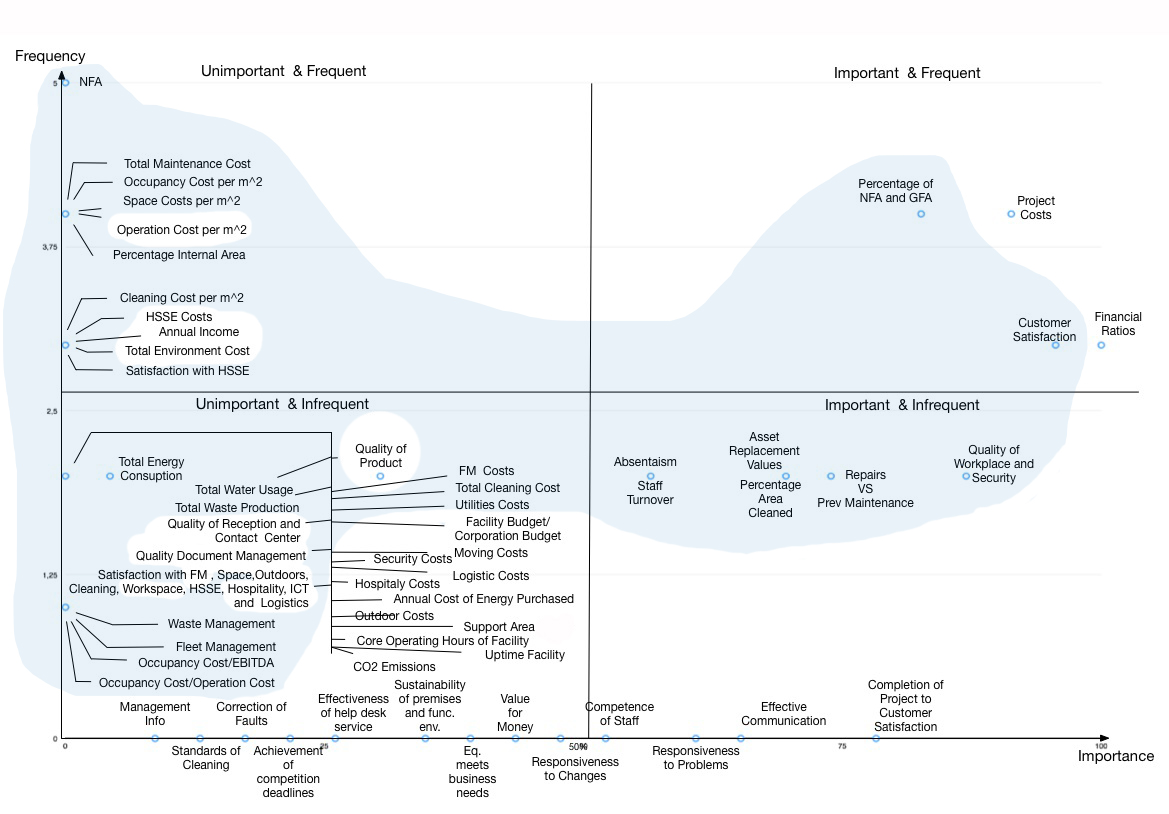
\includegraphics[width=1.1\textwidth]{img/importanceXfrequency10.jpg}
  %\end{adjustwidth}
  \caption{FM KPIs organized according to frequency and importance. Shaded area represents the options of an FM expert.}
  \label{fig:importanceXfrequency}
\end{figure}
In order to understand which were the most important KPIs for FM, it was needed to cross data between the various scientific literature and the existing solutions.
The Figure \ref{fig:importanceXfrequency} represents the information in tables \ref{tb:23KPIimportanceOrder}, \ref{tb:ListSpacialFinancialKPIpapers} and the KPIs given by the FM expert. In it, it is possible to visualize the most relevant KPIs based on importance and frequency. This graphic was constructed based on a cross-over of the KPIs described on the academic literature and the field experience of the FM expert. 



%Having regard the practical and theoretical level, the indicators on the shaded area of the figure are the best ones to compose the final list of indicators and will be used in the proposed solution.

 %So, of KPIs presented in Tables \ref{tb:ListSpacialFinancialKPIpapers} and \ref{tb:Resto2ListKPIpapers}, we could select only the most important ones. These KPIs are presented in Table \ref{tb:ListFinalKPI} and are the representatives of each dimension. 


%Some indicators have the same correspondent point on the graphic: {\bf [Note A] } Total Maintenance Cost, Occupancy Cost per $m^2$, Space Cost per $m^2$ and Operation Cost per $m^2$, {\bf [Note B]} Cleaning Cost per $m^2$, HSSE Costs, Annual Income, Total Environment Cost and Satisfaction with HSSE, {\bf [Note C]} Total Cleaning Cost, FM Costs, Utilities Costs, Facility Budget/Corporation Budget, Moving Costs, Security Costs, Logistic Costs, Hospitality Costs, Annual Cost of Energy Purchased, Outdoor Costs, Support Area, Core Operating Hours of Facility, Uptime Facility, CO2 Emissions, Total Water Usage, Total Waste Production, Quality of Cleaning, Quality of Reception and Contact Center, Quality of Document Management, Satisfaction with FM, Space, Outdoors, Cleaning, Workspace, HSSE,  Hospitality, ICT and Logistics, {\bf [Note D]} Occupancy Costs/Operation Costs, Occupancy Costs/EBITDA, Fleet Management and Waste Management. The indicators within the line are the ones chosen to be used on this document solution.

In order to be simpler to evaluate, a first iteration of the solution should use a short list of KPIs \cite{Costa2004}. The proposed list of KPIs for this project can be seen on Table \ref{tb:ListFinalKPI}.

\begin{table}[h!]%[t!]
	\vspace{0cm}
	\begin{adjustwidth}{-0.5cm}{0cm} 
	\resizebox{13cm}{!} {
	\begin{tabular}{llp{7cm}l}
		\hline
		 {\bf Indicator} &  {\bf Units/mo} & {\bf Description} \\
		\hline
		{\bf Financial Indicators} & & \\
		Total Cleaning Cost 				& \euro &  Sum of all cleaning costs \\
		Cleaning Cost per $m^2$ 			& \euro/$m^2$ &  Total Cleaning Cost/Net Room Area OR Total Cleaning Costs/Net Floor Area\\
		Total Maintenance Cost 				& \euro &  Sum of costs of maintenance for electricity equipment, HVAC, elevators, escalators, generators, UPS, ICT maintenance, etc\\  
		FM Costs 							& \euro &  Costs of FM department OR FM outsourcing \\
		Utility Costs 						& \euro  & Sum of costs for water, electricity, oil, gas and others \\
		Space Costs per $m^2$ 				& \euro/$m^2$ & Total Space Costs/Net Floor Area\\ 
		Occupancy Cost 						& \euro/$m^2$ & Total Occupancy Cost/Net Floor Area \\
		Occupancy Cost per Operation Costs & \% & (Occupancy Cost/Total Operation Costs)*100 \\
		Occupancy Cost per EBITDA & \% & (Occupancy Cost/Earning Before Interest, Taxes, Depreciation and Amortization)*100\\
		\hline

		{\bf Spacial Indicators} & & \\
		Net Floor Area per FTE				& $m^2$/FTE & Net Floor Area/Number of FTE personnel \\
		Percentage Net Floor Area 			& \% & (Net Floor Area/Total Level Area)x100 \\
		Percentage Internal Area			& \% & (Internal Area/Total Level Area)x100 \\
		Percentage Gross Floor Area 		& \% & (Gross Floor Area/Total Level Area)x100 \\
		\hline
		{\bf Maintenance/Cleaning Indicators} & &  \\
		Repairs VS Preventive Maintenance (by specialty)						& \% & (Number of Corrective Maintenance per month/Number of Preventive Maintenance per month)x100 \\
		Asset Replacement Values (by specialty)												& \% & (Annual Maintenance Cost/Maintained Assets Replacement Value)x100\\
		Percentage of Area Cleaned 												& \% & Area Cleaned/Net Floor Area \\
		\hline
		{\bf Productivity Indicators} & & \\
		Staff Turnover 	 			& \% & (Number of Employee Departures (FTE)/Average Number of Staff Members (FTE) Employed)x100\\
		Absenteeism  				& \% & (Total Days Lost/Total Possible Days Worked)x100 \\
		\hline

		{\bf Environmental Indicators} & & \\
		%CO2 emissions 						& tones/mo &  \\
		Total Energy Consumption	 		& kWh & \\
		Total Water Usage					& $m^3$ & \\
		Total Waste Production 				& tones & \\
		%Health and safety and environment 	&  & ? \\
		\hline
		 {\bf Service Quality Indicators} &  &  \\ 
		Quality of Cleaning							&  & Values Obtained Through Audits or Questionnaires \\
		Quality of Workplace 						&  & Values Obtained Through Audits or Questionnaires \\
		Quality of Security 						&  & Values Obtained Through Audits or Questionnaires \\
		\hline
		{\bf Satisfaction Indicators} & & \\
		Client Satisfaction 			& \% & Values Obtained Through Questionnaires \\
		Satisfaction with Space			& \% & Values Obtained Through Questionnaires \\
		Satisfaction with Cleaning 		& \% & Values Obtained Through Questionnaires \\
		Satisfaction with HSSE			& \% & Values Obtained Through Questionnaires \\
		\hline
	\end{tabular}
	}
	\end{adjustwidth}
\caption{List of Final Normalized KPIs that will be used on final solution, after validation by several FM experts.}
\label{tb:ListFinalKPI}
\end{table}
			